%%%%%%% Chapter template %%%%%%%%%%

\chapter{Template}
\thispagestyle{empty}

\section{Section}
\begin{figure}[htb!]
	\centering
	\includegraphics[width=6cm]{img/thing.jpg}
	\caption{This graphic visualizes something really interesting.}
	\label{fig:dummy}
\end{figure}
\paragraph{Paragraph - Formulas}
This is a regular formula $ x^{2 \pi}$ and a formula with a linebreak 
\[ \min_{\mathbf{Q}} \sum_i \left\| \mathbf{A}_i \mathbf{Q} - \mathbf{P}_i(\mathbf{A}_i \mathbf{Q}) \right\|^2_\mathrm{F} \]
Another option:
$$
x = -\frac{p}{2} \pm \sqrt{(\frac{p}{2})^2 -q}
$$

Or also as a numbered equation:
\begin{equation}
	x = -\frac{p}{2} \pm \sqrt{(\frac{p}{2})^2 -q}
\end{equation}

Or in alignment with multiple equations:
\begin{align*}
	\psi(x,y) = [lfp R, v. &(v = y) \vee \\
	&(V_0 v \wedge \exists v' (Evv' \wedge Rv')) \vee\\
	&(V_1 v \wedge \forall v' (Evv' \rightarrow Rv'))](y)
\end{align*}

\[F(X) = \begin{cases}
	A & \mbox{ for } X = \emptyset\\
	X & \mbox{ otherwise}
\end{cases}\]

Something fancy:
\begin{align*}
	\pi  &= \overbrace{11}^{x_0}|\overbrace{0}^{x_1}|\overbrace{101}^{x_2}|\overbrace{100 0}^{x_3}|\overbrace{101}^{x_4}|\overbrace{00 0}^{x_5}|\overbrace{1}^{x_6}|\ldots\\
	\pi' &= \underbrace{11}_{x_0'}|\underbrace{1 010}_{x_1'}|\underbrace{011}_{x_2'}|\underbrace{1 010}_{x_3'}|\underbrace{11}_{x_4'}|\underbrace{1 0}_{x_5'}|\ldots
\end{align*}

and with some text in same row:
\begin{equation*}
	w^T \phi(x) + b =0 \quad \Rightarrow \text{Nonlinear Classifier in} \; R^D
\end{equation*}

% for better overview chapters can be included from separate files
\input{extern/external.tex}

\section{Some drawing and tables}
A simple automaton drawn with tikz nodes.\\ 
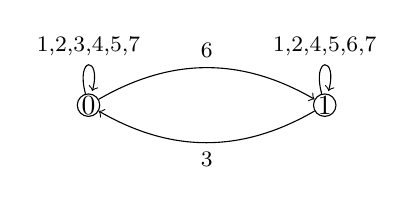
\begin{tikzpicture}
	[state/.style ={draw, circle, inner sep = 0pt}]
	\node[state] (0) at (0,0) {$0$};
	\node[state] (1) at (3,0) {$1$};
	\path[->] (0) edge[loop above, font = \footnotesize] node {1,2,3,4,5,7} (0)
	edge[bend left, font = \footnotesize] node[above] {6} (1)
	(1) edge[loop above] node[font = \footnotesize,above] {1,2,4,5,6,7} (1)
	edge[bend left] node[font = \footnotesize, below] {3} (0);
\end{tikzpicture}

A table containing some information:
\begin{center}
	\begin{tabular}{c|c|c}
		\ & $\ell$ & $r$\\
		\hline
		$t$ & $(0, 0)$ & $(0, 0)$\\
		\hline
		$b$ & $(0, 0)$ & $(1, 1)$
	\end{tabular}
\end{center}
And an annotated table:
\[ \begin{blockarray}{ c c c c}
	& denied & granted & \sum \\
	\begin{block}{ c(cc)c }
		protected & a & b &  n_{p}  \\
		unprotected & c & d & n_{u} \\
	\end{block}
	\begin{block}{c c c c}
		\sum & m_d & m_g & n\\
	\end{block}
\end{blockarray}\]%

Plotting can also be done in a tikz environment:\\
\begin{tikzpicture}[scale = 0.6]
	\begin{axis}[every axis plot post/.append style={
			mark=none,domain=1:10,samples=50,smooth},
		axis x line*=bottom, % no box around the plot, only x and y axis
		axis y line*=left, % the * suppresses the arrow tips
		ylabel = {$Pr(\lambda' = x)$},
		xtick={5},
		minor xtick={2,4,...,10},
		xticklabels = {$\lambda$},
		grid = major, ymajorgrids = false,
		x tick label style={black},
		enlarge y limits={abs value=.15, upper}, ]
		\addplot {gauss(5,0.75)};
		\legend{Distribution of the sample mean}
	\end{axis}
	\pgftransformshift{\pgfpoint{10cm}{0cm}}
	\begin{axis}[every axis plot post/.append style={
			mark=none,domain=1:10,samples=50,smooth},
		axis x line*=bottom, % no box around the plot, only x and y axis
		axis y line*=left, % the * suppresses the arrow tips
		ylabel = {$Pr(\lambda' = x)$},
		xtick={3.33,5},
		minor xtick={2,4,...,10},
		xticklabels = {$\frac{2}{3}\lambda$,$\lambda$},
		grid = major, ymajorgrids = false,
		x tick label style={black},
		enlarge y limits={abs value=.15, upper}, ]
		\addplot[color = red] {gauss(5*0.666,0.75)};
		\legend{Mixed strategy}
	\end{axis}
\end{tikzpicture}